\documentclass{article}
\usepackage{xunicode}
\usepackage{fontspec}
\usepackage[frenchb]{babel}
\usepackage{graphicx}
\usepackage{listings}
\usepackage[T1]{fontenc}
\usepackage{kpfonts}


\renewcommand*{\familydefault}{\sfdefault}

\renewcommand{\nobreakspace}{\nobreak\ }



\title{SUAPS}
\author{Clotilde \textsc{Massot} \and Alexandre \textsc{Garnier} \and Chimène Gaby \textsc{Nya Ngaha} \and Julien \textsc{Durillon}}

\begin{document}

\maketitle

\section{Analyse}

	\subsection{Utilisateurs}
		La population des utilisateurs du point de vue du logiciel est sensiblement homogène.
	
	\subsection{Tâches}
	
\section{Conception de l'interface}

	Une fois définie la population des utilisateurs cible, vient la définition et la conception d'une interface efficace. Ici l'efficacité consiste en une solution à même d'offrir les fonctions attendues des utilisateurs dans une interface adaptée à leur connaissance de l'environnement applicatif.

	\subsection{Concept d'interaction}
	
	En celà, il s'agit ici de parvenir à proposer une solution simple et claire à utiliser, de telle sorte que l'accession aux fonctions clés de l'application soient accessibles rapidement et intuitivement.
	
	Dès lors, et afin de proposer une interface potentiellement connue de l'utilisateur, nous avons eu pour idée de s'inspirer de l'application AlloCiné pour Android. Notamment l'analogie entre la recherche et l'affichage de films d'un côté, de sports d'un autre, s'est imposée d'elle-même.
	
	\begin{figure}[ht]
		\centering
		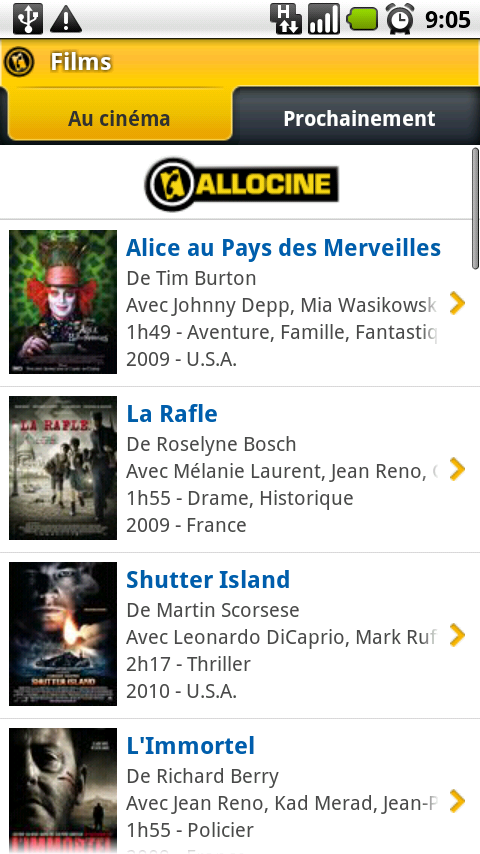
\includegraphics[width=0.5\textwidth]{allocine.png}
		\caption{Application AlloCiné : liste de films.}
		\label{fig:allocine}
	\end{figure}
	
	En outre, reprendre ainsi une interface que connaît l'utilisateur offre l'avantage de répondre à ses habitudes, automatisme	et exigences.
	
	\subsection{Écrans-clés}
	
	
	
	\subsection{Look and feel}
	
	
	
	\subsection{Prototypage}



\end{document}